\documentclass[conference]{style/IEEEtran}
\IEEEoverridecommandlockouts
\usepackage{cite}
\usepackage{amsmath,amssymb,amsfonts}
\usepackage{algorithmic}
\usepackage{graphicx}
\usepackage{textcomp}
\usepackage{xcolor}
\def\BibTeX{{\rm B\kern-.05em{\sc i\kern-.025em b}\kern-.08em
    T\kern-.1667em\lower.7ex\hbox{E}\kern-.125emX}}
\usepackage[sorting=none]{biblatex}
\addbibresource{references/references.bib}
    
\begin{document}
\title{A methodological framework to enable the roaming agreement digitalization: An NLP-based approach\\}

\maketitle

\begin{abstract}
This document is a model and instructions for \LaTeX.
This and the IEEEtran.cls file define the components of your paper [title, text, heads, etc.]. *CRITICAL: Do Not Use Symbols, Special Characters, Footnotes, 
or Math in Paper Title or Abstract.
\end{abstract}

\begin{IEEEkeywords}
component, formatting, style, styling, insert
\end{IEEEkeywords}

\section{Introduction}
The roaming service maintains the persistent connectivity of subscribers in different networks and locations. Roaming describes the capability of a subscriber to access mobile services offered by the visited public mobile network (VPMN) through the home public mobile network (HPMN), when roaming outside the coverage range of the HPMN \cite{Tanaka2013}. However, before ensuring persistent connectivity the Mobile Network Operators (MNOs) must reach an agreement regarding the technical, commercial and legal relationships known as the Roaming Agreement (RA).

In order to standardize technical, commercial and legal aspects of RA, the GSM Association broadly outlines the content of such RA in standardized form for its members \cite{Ferwerda2018}. Reference \cite{ROCCO2017} provides a list of the most commonly used GSMA standards, which are summarized bellow: (1) AA.12 constitutes the permanent reference document; (2) AA.13 contains the common annexes with operational information (e.g., information on tap file, billing data, settlement procedure, customer care, fraud, etc.) and (3) AA.14 involves the individual annexes containing information about the operator (e.g., contact details of the roaming team, fraud team, IREG team, TADIG team, etc.).

While it is true that it is not mandatory to follow the standards proposed by GSMA, according to authoritative voices in the field of negotiating RA drafting, most MNOs follow them strictly \cite{ROCCO2017a}. Therefore, a first point to consider in the RA drafting is how far it is deviated from the GSMA's proposed standards. Thus, during the drafting process of the agreement, the parties should analyze the sub-articles contained in the GSMA standard templates to determine whether:

\begin{enumerate}
\item Specify the value of certain \textit{variables} that are found in a certain text, such as dates, names of entities, amounts and others.

\item Leave an article/sub-article as found in the template thereby establishing a \textit{standard clause}.

\item Introduce certain \textit{variations} in the articles/sub-articles, by changing \textit{variables}, e.g., MNO commercial name, dates, penalties, currencies and so on with respect to the original text, i.e., the GSMA standard templates.

\item Introduce completely new articles/sub-articles that respond to particular interests by constituting \textit{customized texts}.

\end{enumerate}

However, a successful RA drafting goes through a complex negotiation process in which, currently the parties, i.e. the MNOs, still use asynchronous flows such as email or even regular mail for information exchange. Since these processes lack transparency, which can result in the violation of the RA by MNOs, it is necessary to provide a transparent digitalization system for RA drafting negotiations. For this reason, this paper proposes the use of Natural Language Processing (NLP) as an engine to digitize the legal text as a starting point of a digitization process of negotiation procedures for a transparent drafting of Roaming Agreements. The NLP engine analyzes articles and sub-articles of the RA determining the existence of variables, variations, standard clauses and customized texts. For this purpose, the NLP engine relies on the one hand, on NLP techniques such as Named Entity Recognition (NER) and Part of Speech (POS) using the unstructured data information discovery tool \textit{Amazon Comprehend} and, on the other hand, by establishing an comprehensive comparison between texts based on \textit{similarity} determination techniques. The procedures for integrating tools, NLP techniques, pre-processing and post-processing constitute a methodological framework designed for the use case and included within an unstructured text processing tool. This article includes not only the design phase, but also the implementation and evaluation of the tool.

The rest of this manuscript is structured as follows: Section 2 reviews both the attempts at transparent digitalization of roaming agreements and existing NLP techniques-based text processing systems as part of related work. Section 3 establishes the designed methodology. The implementation of our system are described in Section 4. Section 5 discusses the results of conducted experiments. Finally, the conclusions of the manuscript are included in Section 6.

\section{Related work}

Both in the scientific literature and in business environments there are important approaches to RA digitalization. Thus, the reference \cite{9369516} proposes a dynamic RA between the Local 5G Operator and the MNO. The interaction between the two entities takes place through an Ethereum based platform. A second approach focuses uniquely on the billing of the services obtained as a result of the RA \cite{9024541}. This agreement is incorporated as part of a smart contract so the work contributes significantly to the digitalization process of the agreement, allowing for a faster, more seamless process in which payments can be requested and obtained quickly due to less need for manual intervention. The contextualization of this system in the business environment is proposed by important MNOs such as Telefonica, Deutsche Telekom and Vodafone which use blockchain for Roaming settlement within the framework of the RA between the parties \cite{Huillet2020}. Despite the value of these contributions from a RA implementation perspective, they are not within the context of a transparent digitalization to improve the negotiation process for the effective drafting of the roaming agreement. 

Additionally, the scientific literature addresses text processing systems based on nlp techniques in domains such as judiciary. Thus, the reference \cite{8487847} addresses the process of digitalization in the judicial sectors from archives of judicial records for which the authors have designed a text analysis tool that includes grammatical analysis of documents in English based on NLP techniques. This linguistic analysis attempts to find the appropriate meaning of terms within a document. In addition, the reference \cite{9138070} applies NLP-based processing techniques for information retrieval from spreadsheets and describes technologies for storing and retrieving database information. NLP techniques such as sentence tokenization, word tokenization, removing stopwords and lemmatization are part of the parsing stage of the work. Finally, authors of reference \cite{9104105} propose a model for implementing sentimental analysis using Amazon Comprehend. This system performs an audio-to-text transcription and then performs the processing of the obtained text. Although these studies  constitute a relevant part of related work, e.g., by integrating useful tools such as Amazon Comprehend or detailing the use of techniques such as tokenization, the scientific literature does not address scenarios for the telecommunication field and even less in the context of a transparent digitalization of the roaming agreement. Therefore, we can affirm that our work introduces a topic with a high degree of novelty.

\section{NLP Engine methodology}
Overall, the logic designed for the NLP engine follows two approaches: \textit{detection} and \textit{comparison}. While \textit{detection} has words as its basic processing unit, \textit{comparison} has sub-articles as its basic processing unit. \textit{Detection} represents the capability to locate \textit{variables} in a text file, i.e., the Roaming Agreement. \textit{Comparison} represents the capacity to find \textit{similarities} and differences between the sub-articles present in the Roaming Agreement with respect to the sub-articles present in the GSMA standard template. For example, while an almost total coincidence between texts at the sub-article level represents a \textit{standard clause}, an almost null coincidence between texts (or simply the non-existence of a sub-article of the GSMA standard template in the Roaming Agreement) represents a \textit{customized text}. Thus, the intermediate case is represented by the \textit{variation} in which there is a high coincidence between sub-articles and the existing differences are given by the presence of \textit{variables} such as the commercial name of a MNO and the start date of the agreement. The technologies that enable both \textit{detection} and \textit{comparison} are discussed below as part of the \textit{background}. The third section integrates tools, NLP techniques, pre-processing and post-processing as part of the designed methodology.

\subsection{Amazon comprehend}
In short, \textit{Amazon Comprehend} is a service that uses NLP techniques to extract insights about the content document by recognizing  the  entities,  key  phrases,  language,  sentiments,  and  other  common  elements  in  a  text \cite{AWS2021}. The capabilities that \textit{Amazon Comprehend} integrates are key in the \textit{detection} approach.

\subsection{Similarity Analysis}
Similarity is used to compare different types of data, so it is a resource used for pattern classification, clustering and information retrieval problems \cite{7429408}. Therefore, the similarity falls within the comparison approach. In this regard, our work distinguishes between two types of similarities: Jaccard similarity and Cosine similarity \cite{Gupta2018}. While the first one is established as the size of the intersection divided by the size of the union of two sets, the second one implies the determination of the cosine of the angle between two vectors.

\subsection{Designed Methodology}
Define abbreviations and acronyms the first time they are used in the text.

\section{Implemented System}
The Fig.~\ref{fig1} shows the overall architecture of the NLP engine integrated in a docker infrastructure that includes 3 parts. First, the input files include the Roaming Agreement text file as well as the GSMA standard templates. The processing layer includes the logic associated with the NLP engine, i.e. the implementation of the designed methodology. The output file constitutes a JavaScript Object Notation (JSON) file populated with the classification of articles and sub-articles as \textit{standard clauses}, \textit{customized texts} and \textit{variations}. Each article includes the set of \textit{variables} it contains and each sub-article contains the specific \textit{variable} detected as long as it has been classified as a variation.

\begin{figure}[htbp]
\centerline{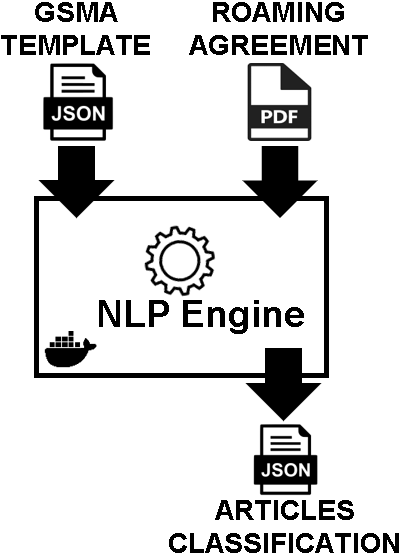
\includegraphics[width=0.23\textwidth]{images/NLP_Engine.png}}
\caption{NLP Engine overall architecture.}
\label{fig1}
\end{figure}

Regarding the input and output files, these are associated to the container through volumes. In addition, the NLP Engine has been developed as a Python v3.8 based library and therefore must be imported and run from an entry point. Although the NLP Engine constitutes a library, it must in turn integrate other libraries, among which boto3 \cite{boto3}. Boto3 is an Software Development Kit (SDK) for Python, created and supported by Amazon Web Services (AWS). The NLP Engine imports the service associated to Amazon Comprehend. Other library imported into NLP Engine library is PyMuPDF (\cite{PyMuPDF}), which is used by the NLP Engine to extract headers and footers from the PDF files. Therefore, the docker image built for the NLP Engine must not only install the NLP Engine library, but must also install the libraries it imports.

\section{Discussion of Results}
Since PDF, i.e., input files of the NLP Engine architecture consist of unstructured text and for instance, undesired characters may remain despite text parsing, it is mandatory determine the \textit{accuracy} of the results obtained once the output JSON file has been populated. For this purpose, two types of experiments have been conducted to determine the \textit{accuracy} of the results. On the one hand, a simple inspection at sub-article level and on the other hand, a verification based on symbol comparison. The tests will be performed on two Roaming Agreements sample of the MNOs Proximus and Orange \cite{proximus}. Each experiment is described below and the results obtained are discussed in the same section.

\subsection{Accuracy determination based on a simple inspection at sub-article level}
The first accuracy analysis consists of determining by simple inspection, i.e., human-eye inspection, whether each sub-article of the roaming agreement constitutes a variation, a standard clause or a customized text with respect to the GSMA standard template. Additionally, the detected variables are analyzed. The results obtained are then compared with the values populated in the NLP Engine output file, for the same articles. Considering that the results obtained from the simple inspection constitute the observations and the values collected from the article and sub-article classification file constitute the predicted values, it is considered for each item, i.e., variable, variation, standard clause and custom text:
\begin{enumerate}
\item True Positive is when the item is observed and predicted.
\item True Negative is when the item is observed but not predicted.
\item False Positive is when the item is not observed but still predicted.
\item False Negative is when the item is neither observed nor predicted..
\end{enumerate}

The following confusion matrices allow us to analyze the results for each roaming agreement:

\subsection{Accuracy determination based on symbol comparison}
The second accuracy analysis involves establishing a comparison between the sub-articles populated in the output file with respect to the sub-articles existing in the input file containing the Roaming Agreements. For that purpose, the text comparison tool Countwordsfree(\cite{countwordsfree}) is used manually copying sub-article by sub-article. For each sub-article is determined:

 \begin{enumerate}
\item Common percentage of words between compared sub-articles.
\item Difference percentage of words between compared sub-articles.
\item Common words between compared sub-articles.
\item Difference words between compared sub-articles.
\end{enumerate}

The following radar plots allow us to analyze the results for each roaming agreement:

\section{Conclusions}
Considering that the proposed NLP Engine constitutes a part of a project that has as main objective of transforming the current Telecommunication Roaming Agreement drafting and negotiation process into a digitalized version based on the transparency promoted by blockchain technology, future research works include the design, development and evaluation of the rest of the sub-systems, as well as the integration of the NLP Engine part. 

\printbibliography

\vspace{12pt}

\end{document}
